\chapter{Chapter V}

\lettrine{H}{ath} not a Jew eyes? Hath not a Jew hands, organs,
dimensions, senses,
affections, passions? Fed with the same food, hurt with the same
weapons, subject to the same diseases, healed by the same means, warmed
and cooled by the same winter and summer, as a Christian is? --Merchant
of Venice

Oswald, returning, whispered into the ear of his master, ``It is a Jew,
who calls himself Isaac of York; is it fit I should marshall him into
the hall?''

``Let Gurth do thine office, Oswald,'' said Wamba with his usual
effrontery; ``the swineherd will be a fit usher to the Jew.''

``St Mary,'' said the Abbot, crossing himself, ``an unbelieving Jew, and
admitted into this presence!''

``A dog Jew,'' echoed the Templar, ``to approach a defender of the Holy
Sepulchre?''

``By my faith,'' said Wamba, ``it would seem the Templars love the Jews'
inheritance better than they do their company.''

``Peace, my worthy guests,'' said Cedric; ``my hospitality must not be
bounded by your dislikes. If Heaven bore with the whole nation of
stiff-necked unbelievers for more years than a layman can number, we may
endure the presence of one Jew for a few hours. But I constrain no man
to converse or to feed with him.--Let him have a board and a morsel
apart,--unless,'' he said smiling, ``these turban'd strangers will admit
his society.''

``Sir Franklin,'' answered the Templar, ``my Saracen slaves are true
Moslems, and scorn as much as any Christian to hold intercourse with a
Jew.''

``Now, in faith,'' said Wamba, ``I cannot see that the worshippers of
Mahound and Termagaunt have so greatly the advantage over the people
once chosen of Heaven.''

``He shall sit with thee, Wamba,'' said Cedric; ``the fool and the knave
will be well met.''

``The fool,'' answered Wamba, raising the relics of a gammon of bacon,
``will take care to erect a bulwark against the knave.''

``Hush,'' said Cedric, ``for here he comes.''

Introduced with little ceremony, and advancing with fear and hesitation,
and many a bow of deep humility, a tall thin old man, who, however, had
lost by the habit of stooping much of his actual height, approached the
lower end of the board. His features, keen and regular, with an aquiline
nose, and piercing black eyes; his high and wrinkled forehead, and long
grey hair and beard, would have been considered as handsome, had they
not been the marks of a physiognomy peculiar to a race, which, during
those dark ages, was alike detested by the credulous and prejudiced
vulgar, and persecuted by the greedy and rapacious nobility, and who,
perhaps, owing to that very hatred and persecution, had adopted a
national character, in which there was much, to say the least, mean and
unamiable.

The Jew's dress, which appeared to have suffered considerably from the
storm, was a plain russet cloak of many folds, covering a dark purple
tunic. He had large boots lined with fur, and a belt around his waist,
which sustained a small knife, together with a case for writing
materials, but no weapon. He wore a high square yellow cap of a peculiar
fashion, assigned to his nation to distinguish them from Christians, and
which he doffed with great humility at the door of the hall.

The reception of this person in the hall of Cedric the Saxon, was such
as might have satisfied the most prejudiced enemy of the tribes of
Israel. Cedric himself coldly nodded in answer to the Jew's repeated
salutations, and signed to him to take place at the lower end of the
table, where, however, no one offered to make room for him. On the
contrary, as he passed along the file, casting a timid supplicating
glance, and turning towards each of those who occupied the lower end of
the board, the Saxon domestics squared their shoulders, and continued to
devour their supper with great perseverance, paying not the least
attention to the wants of the new guest. The attendants of the Abbot
crossed themselves, with looks of pious horror, and the very heathen
Saracens, as Isaac drew near them, curled up their whiskers with
indignation, and laid their hands on their poniards, as if ready to rid
themselves by the most desperate means from the apprehended
contamination of his nearer approach.

Probably the same motives which induced Cedric to open his hall to this
son of a rejected people, would have made him insist on his attendants
receiving Isaac with more courtesy. But the Abbot had, at this moment,
engaged him in a most interesting discussion on the breed and character
of his favourite hounds, which he would not have interrupted for matters
of much greater importance than that of a Jew going to bed supperless.
While Isaac thus stood an outcast in the present society, like his
people among the nations, looking in vain for welcome or resting place,
the pilgrim who sat by the chimney took compassion upon him, and
resigned his seat, saying briefly, ``Old man, my garments are dried, my
hunger is appeased, thou art both wet and fasting.'' So saying, he
gathered together, and brought to a flame, the decaying brands which lay
scattered on the ample hearth; took from the larger board a mess of
pottage and seethed kid, placed it upon the small table at which he had
himself supped, and, without waiting the Jew's thanks, went to the other
side of the hall;--whether from unwillingness to hold more close
communication with the object of his benevolence, or from a wish to draw
near to the upper end of the table, seemed uncertain.

Had there been painters in those days capable to execute such a subject,
the Jew, as he bent his withered form, and expanded his chilled and
trembling hands over the fire, would have formed no bad emblematical
personification of the Winter season. Having dispelled the cold, he
turned eagerly to the smoking mess which was placed before him, and ate
with a haste and an apparent relish, that seemed to betoken long
abstinence from food.

Meanwhile the Abbot and Cedric continued their discourse upon hunting;
the Lady Rowena seemed engaged in conversation with one of her attendant
females; and the haughty Templar, whose eye wandered from the Jew to the
Saxon beauty, revolved in his mind thoughts which appeared deeply to
interest him.

``I marvel, worthy Cedric,'' said the Abbot, as their discourse
proceeded, ``that, great as your predilection is for your own manly
language, you do not receive the Norman-French into your favour, so far
at least as the mystery of wood-craft and hunting is concerned. Surely
no tongue is so rich in the various phrases which the field-sports
demand, or furnishes means to the experienced woodman so well to express
his jovial art.''

``Good Father Aymer,'' said the Saxon, ``be it known to you, I care not
for those over-sea refinements, without which I can well enough take my
pleasure in the woods. I can wind my horn, though I call not the blast
either a `recheate' or a `morte'--I can cheer my dogs on the prey, and I
can flay and quarter the animal when it is brought down, without using
the newfangled jargon of `curee, arbor, nombles', and all the babble of
the fabulous Sir Tristrem.''\footnote{There was no language which the
Normans more formally
separated from that of common life than the terms of the chase. The
objects of their pursuit, whether bird or animal, changed their name
each year, and there were a hundred conventional terms, to be ignorant
of which was to be without one of the distinguishing marks of a
gentleman. The reader may consult Dame Juliana Berners' book on the
subject. The origin of this science was imputed to the celebrated Sir
Tristrem, famous for his tragic intrigue with the beautiful Ysolte. As
the Normans reserved the amusement of hunting strictly to themselves,
the terms of this formal jargon were all taken from the French
language.}

``The French,'' said the Templar, raising his voice with the
presumptuous and authoritative tone which he used upon all occasions,
``is not only the natural language of the chase, but that of love and of
war, in which ladies should be won and enemies defied.''

``Pledge me in a cup of wine, Sir Templar,'' said Cedric, ``and fill
another to the Abbot, while I look back some thirty years to tell you
another tale. As Cedric the Saxon then was, his plain English tale
needed no garnish from French troubadours, when it was told in the ear
of beauty; and the field of Northallerton, upon the day of the Holy
Standard, could tell whether the Saxon war-cry was not heard as far
within the ranks of the Scottish host as the `cri de guerre' of the
boldest Norman baron. To the memory of the brave who fought
there!--Pledge me, my guests.'' He drank deep, and went on with
increasing warmth. ``Ay, that was a day of cleaving of shields, when a
hundred banners were bent forwards over the heads of the valiant, and
blood flowed round like water, and death was held better than flight. A
Saxon bard had called it a feast of the swords--a gathering of the
eagles to the prey--the clashing of bills upon shield and helmet, the
shouting of battle more joyful than the clamour of a bridal. But our
bards are no more,'' he said; ``our deeds are lost in those of another
race--our language--our very name--is hastening to decay, and none
mourns for it save one solitary old man--Cupbearer! knave, fill the
goblets--To the strong in arms, Sir Templar, be their race or language
what it will, who now bear them best in Palestine among the champions of
the Cross!''

``It becomes not one wearing this badge to answer,'' said Sir Brian de
Bois-Guilbert; ``yet to whom, besides the sworn Champions of the Holy
Sepulchre, can the palm be assigned among the champions of the Cross?''

``To the Knights Hospitallers,'' said the Abbot; ``I have a brother of
their order.''

``I impeach not their fame,'' said the Templar; ``nevertheless---''

``I think, friend Cedric,'' said Wamba, interfering, ``that had Richard
of the Lion's Heart been wise enough to have taken a fool's advice, he
might have staid at home with his merry Englishmen, and left the
recovery of Jerusalem to those same Knights who had most to do with the
loss of it.''

``Were there, then, none in the English army,'' said the Lady Rowena,
``whose names are worthy to be mentioned with the Knights of the Temple,
and of St John?''

``Forgive me, lady,'' replied De Bois-Guilbert; ``the English monarch
did, indeed, bring to Palestine a host of gallant warriors, second only
to those whose breasts have been the unceasing bulwark of that blessed
land.''

``Second to NONE,'' said the Pilgrim, who had stood near enough to hear,
and had listened to this conversation with marked impatience. All turned
toward the spot from whence this unexpected asseveration was heard.

\begin{figure}
    \centering
    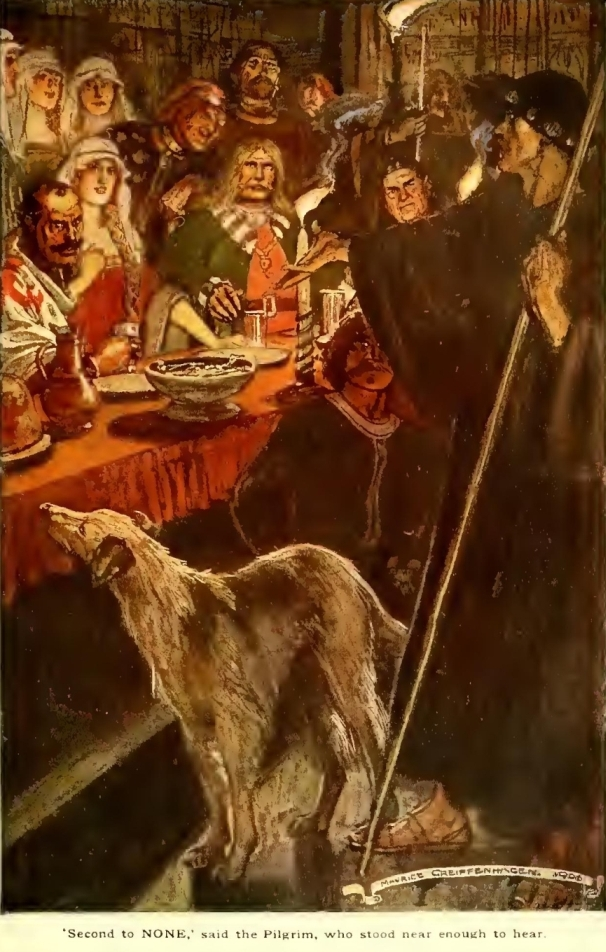
\includegraphics[height=.9\textheight]{ivanhoe/0087m}
    \caption{`Second to \textsc{none},' said the Pilgrim, who stood
    near enough to hear.}
\end{figure}

``I say,'' repeated the Pilgrim in a firm and strong voice, ``that the
English chivalry were second to NONE who ever drew sword in defence of
the Holy Land. I say besides, for I saw it, that King Richard himself,
and five of his knights, held a tournament after the taking of St
John-de-Acre, as challengers against all comers. I say that, on that
day, each knight ran three courses, and cast to the ground three
antagonists. I add, that seven of these assailants were Knights of the
Temple--and Sir Brian de Bois-Guilbert well knows the truth of what I
tell you.''

It is impossible for language to describe the bitter scowl of rage which
rendered yet darker the swarthy countenance of the Templar. In the
extremity of his resentment and confusion, his quivering fingers griped
towards the handle of his sword, and perhaps only withdrew, from the
consciousness that no act of violence could be safely executed in that
place and presence. Cedric, whose feelings were all of a right onward
and simple kind, and were seldom occupied by more than one object at
once, omitted, in the joyous glee with which he heard of the glory of
his countrymen, to remark the angry confusion of his guest; ``I would
give thee this golden bracelet, Pilgrim,'' he said, ``couldst thou tell
me the names of those knights who upheld so gallantly the renown of
merry England.''

``That will I do blithely,'' replied the Pilgrim, ``and without guerdon;
my oath, for a time, prohibits me from touching gold.''

``I will wear the bracelet for you, if you will, friend Palmer,'' said
Wamba.

``The first in honour as in arms, in renown as in place,'' said the
Pilgrim, ``was the brave Richard, King of England.''

``I forgive him,'' said Cedric; ``I forgive him his descent from the
tyrant Duke William.''

``The Earl of Leicester was the second,'' continued the Pilgrim; ``Sir
Thomas Multon of Gilsland was the third.''

``Of Saxon descent, he at least,'' said Cedric, with exultation.

``Sir Foulk Doilly the fourth,'' proceeded the Pilgrim.

``Saxon also, at least by the mother's side,'' continued Cedric, who
listened with the utmost eagerness, and forgot, in part at least, his
hatred to the Normans, in the common triumph of the King of England and
his islanders. ``And who was the fifth?'' he demanded.

``The fifth was Sir Edwin Turneham.''

``Genuine Saxon, by the soul of Hengist!'' shouted Cedric--``And the
sixth?'' he continued with eagerness--``how name you the sixth?''

``The sixth,'' said the Palmer, after a pause, in which he seemed to
recollect himself, ``was a young knight of lesser renown and lower rank,
assumed into that honourable company, less to aid their enterprise than
to make up their number--his name dwells not in my memory.''

``Sir Palmer,'' said Sir Brian de Bois-Guilbert scornfully, ``this
assumed forgetfulness, after so much has been remembered, comes too late
to serve your purpose. I will myself tell the name of the knight before
whose lance fortune and my horse's fault occasioned my falling--it was
the Knight of Ivanhoe; nor was there one of the six that, for his years,
had more renown in arms.--Yet this will I say, and loudly--that were he
in England, and durst repeat, in this week's tournament, the challenge
of St John-de-Acre, I, mounted and armed as I now am, would give him
every advantage of weapons, and abide the result.''

``Your challenge would soon be answered,'' replied the Palmer, ``were
your antagonist near you. As the matter is, disturb not the peaceful
hall with vaunts of the issue of the conflict, which you well know
cannot take place. If Ivanhoe ever returns from Palestine, I will be his
surety that he meets you.''

``A goodly security!'' said the Knight Templar; ``and what do you
proffer as a pledge?''

``This reliquary,'' said the Palmer, taking a small ivory box from his
bosom, and crossing himself, ``containing a portion of the true cross,
brought from the Monastery of Mount Carmel.''

The Prior of Jorvaulx crossed himself and repeated a pater noster, in
which all devoutly joined, excepting the Jew, the Mahomedans, and the
Templar; the latter of whom, without vailing his bonnet, or testifying
any reverence for the alleged sanctity of the relic, took from his neck
a gold chain, which he flung on the board, saying--``Let Prior Aymer
hold my pledge and that of this nameless vagrant, in token that when the
Knight of Ivanhoe comes within the four seas of Britain, he underlies
the challenge of Brian de Bois-Guilbert, which, if he answer not, I will
proclaim him as a coward on the walls of every Temple Court in Europe.''

``It will not need,'' said the Lady Rowena, breaking silence; ``My voice
shall be heard, if no other in this hall is raised in behalf of the
absent Ivanhoe. I affirm he will meet fairly every honourable challenge.
Could my weak warrant add security to the inestimable pledge of this
holy pilgrim, I would pledge name and fame that Ivanhoe gives this proud
knight the meeting he desires.''

A crowd of conflicting emotions seemed to have occupied Cedric, and kept
him silent during this discussion. Gratified pride, resentment,
embarrassment, chased each other over his broad and open brow, like the
shadow of clouds drifting over a harvest-field; while his attendants, on
whom the name of the sixth knight seemed to produce an effect almost
electrical, hung in suspense upon their master's looks. But when Rowena
spoke, the sound of her voice seemed to startle him from his silence.

``Lady,'' said Cedric, ``this beseems not; were further pledge
necessary, I myself, offended, and justly offended, as I am, would yet
gage my honour for the honour of Ivanhoe. But the wager of battle is
complete, even according to the fantastic fashions of Norman
chivalry--Is it not, Father Aymer?''

``It is,'' replied the Prior; ``and the blessed relic and rich chain
will I bestow safely in the treasury of our convent, until the decision
of this warlike challenge.''

Having thus spoken, he crossed himself again and again, and after many
genuflections and muttered prayers, he delivered the reliquary to
Brother Ambrose, his attendant monk, while he himself swept up with less
ceremony, but perhaps with no less internal satisfaction, the golden
chain, and bestowed it in a pouch lined with perfumed leather, which
opened under his arm. ``And now, Sir Cedric,'' he said, ``my ears are
chiming vespers with the strength of your good wine--permit us another
pledge to the welfare of the Lady Rowena, and indulge us with liberty to
pass to our repose.''

``By the rood of Bromholme,'' said the Saxon, ``you do but small credit
to your fame, Sir Prior! Report speaks you a bonny monk, that would hear
the matin chime ere he quitted his bowl; and, old as I am, I feared to
have shame in encountering you. But, by my faith, a Saxon boy of twelve,
in my time, would not so soon have relinquished his goblet.''

The Prior had his own reasons, however, for persevering in the course of
temperance which he had adopted. He was not only a professional
peacemaker, but from practice a hater of all feuds and brawls. It was
not altogether from a love to his neighbour, or to himself, or from a
mixture of both. On the present occasion, he had an instinctive
apprehension of the fiery temper of the Saxon, and saw the danger that
the reckless and presumptuous spirit, of which his companion had already
given so many proofs, might at length produce some disagreeable
explosion. He therefore gently insinuated the incapacity of the native
of any other country to engage in the genial conflict of the bowl with
the hardy and strong-headed Saxons; something he mentioned, but
slightly, about his own holy character, and ended by pressing his
proposal to depart to repose.

The grace-cup was accordingly served round, and the guests, after making
deep obeisance to their landlord and to the Lady Rowena, arose and
mingled in the hall, while the heads of the family, by separate doors,
retired with their attendants.

``Unbelieving dog,'' said the Templar to Isaac the Jew, as he passed him
in the throng, ``dost thou bend thy course to the tournament?''

``I do so propose,'' replied Isaac, bowing in all humility, ``if it
please your reverend valour.''

``Ay,'' said the Knight, ``to gnaw the bowels of our nobles with usury,
and to gull women and boys with gauds and toys--I warrant thee store of
shekels in thy Jewish scrip.''

``Not a shekel, not a silver penny, not a halfling--so help me the God
of Abraham!'' said the Jew, clasping his hands; ``I go but to seek the
assistance of some brethren of my tribe to aid me to pay the fine which
the Exchequer of the Jews have imposed upon me--Father Jacob be my
speed! I am an impoverished wretch--the very gaberdine I wear is
borrowed from Reuben of Tadcaster.''\footnote{In those days the Jews were
subjected to an Exchequer,
specially dedicated to that purpose, and which laid them under the most
exorbitant impositions.--L. T.}

The Templar smiled sourly as he replied, ``Beshrew thee for a
false-hearted liar!'' and passing onward, as if disdaining farther
conference, he communed with his Moslem slaves in a language unknown to
the bystanders. The poor Israelite seemed so staggered by the address of
the military monk, that the Templar had passed on to the extremity of
the hall ere he raised his head from the humble posture which he had
assumed, so far as to be sensible of his departure. And when he did look
around, it was with the astonished air of one at whose feet a
thunderbolt has just burst, and who hears still the astounding report
ringing in his ears.

The Templar and Prior were shortly after marshalled to their sleeping
apartments by the steward and the cupbearer, each attended by two
torchbearers and two servants carrying refreshments, while servants of
inferior condition indicated to their retinue and to the other guests
their respective places of repose.
